\documentclass[12pt,a4paper,onecolumn]{article}
\input{packages}
\input{macros}

% ------------------------ General informations --------------------------------
\title{Math M2 Probabilistic graphical models 2017/2018}
\author{Vincent Matthys}
\graphicspath{{images/}}
% ------------------------------------------------------------------------------

\begin{document}
\begin{tabularx}{0.8\textwidth}{@{} l X r @{} }
	{\textsc{Master MVA}}       &  & \textsc{Rapport expérimental} \\
	\textsc{3D Computer Vision} &  & {Vincent Matthys}             \\
\end{tabularx}
\vspace{1.5cm}
\begin{center}
	\rule[11pt]{5cm}{0.5pt}

	\textbf{\LARGE \textsc{Détecteurs de coins d'Harris}}
	\vspace{0.5cm}\\
	Vincent Matthys\\
	\rule{5cm}{0.5pt}
	\vspace{1.5cm}
\end{center}

Ce projet consiste en un développement dans l'élaborateur d'un détecteur de coins d'Harris, ainsi que d'un rafinement des détections par \textit{adaptive non-maximal suppression}. Le rapport qui suit regroupe différentes observations quand à son utilisation sur différentes images, avec différents paramètres et dans des conditions différentes, ceci dans un soucis d'évaluation qualitative du progamme délivré.

\tableofcontents
\section{Différentes scènes}

En figure~\ref{fig_1} sont présentés 4 résultats donnés par le détecteurs de coins de Harris implémenté, sur des images de taille comparable, avec les paramètres suivants :
\begin{itemize}
	\item \( \sigma_d = 1\) écart-type du noyau de convolution pour la dérivation.
	\item \( \sigma_i = 1\) écart-type de la fenêtre gaussienne de lissage des images produits.
	\item \( \kappa = 0.05\) constante multiplicative de la fonction de réponse
	\item \( threshold = 0.01\) seuil global (en fonction de la réponse maximale) en deça duquel aucune réponse n'est considérée.
	\item \(local = 3\) délimite la fenêtre de recherche du maximum local
	\item \(c = 0.7\) seuillage au delà duquel le point est automatiquement détecté.
	\item \( b = 50\) nombre de détections souhaité.
\end{itemize}
\begin{figure}[H]
	\centering
	\begin{subfigure}[b]{\textwidth}
		\centering
		\includegraphics[height = 0.20\textheight]{1_bouc}
		\subcaption{Image Bouc, 495x495 pixels : 1265 coins détectés avant anms, 50 après}
		\label{fig_1_bouc}
	\end{subfigure}
	\begin{subfigure}[b]{\textwidth}
		\centering
		\includegraphics[height = 0.20\textheight]{1_cameraman}
		\subcaption{Image Cameraman, 256x256 pixels : 156 coins détectés avant anms, 50 après}
		\label{fig_1_cameraman}
	\end{subfigure}
	\begin{subfigure}[b]{\textwidth}
		\centering
		\includegraphics[height = 0.20\textheight]{1_lena}
		\subcaption{Image Lena, 512x512 pixels : 326 coins détectés avant anms, 50 après}
		\label{fig_1_lena}
	\end{subfigure}
	\begin{subfigure}[b]{\textwidth}
		\centering
		\includegraphics[height = 0.20\textheight]{1_room}
		\subcaption{Image Room, 512x512 pixels : 407 coins détectés avant anms, 50 après}
		\label{fig_1_room}
	\end{subfigure}
	\caption{Détecteurs de coins d'Harris sur différentes scènes. Colonne de gauche, sans \textit{adaptative non-maximal supression} ; colonne de droite, avec \textit{adaptative non-maximal supression}}
	\label{fig_1}
\end{figure}
En figure~\ref{fig_1_bouc}, on constate un très grand nombre de coins détectés, 5 fois supérieur aux autres images de même taille. Ceci est très bien expliqué par la géométrie du circuit représenté dans l'image, composé essentiellement de lignes ayant une forte réponse dans les images produits. Dans les 3 autres images~\ref{fig_1_cameraman}~\ref{fig_1_lena}~\ref{fig_1_room}, le nombre de coins détectés est sensiblement identique, si on le raméne à la taille de l'image. On constate légèrement plus de détections dans l'image Room pour les mêmes raisons que l'image Bouc, dans le carré de tissu présentant des lignes non totalement horizontales répondant fortement dans les images produits.

Une autre constatation importante est la localisation des détections, qui se situent dans les zones non constantes par morceaux, \textit{a fortiori} très constratées. Ceci est encore une fois expliqué par la réponse nulle de telles zones dans les images produits.

Enfin, l'\textit{adaptative non-maximal supression} agit comme attendu, gardant des détections de façon non homogène, dépendante de la densité initiale mais en gardant un support spatial des détections semblable au support spatial avant \textit{adaptative non-maximal supression}.

\section{Différents paramètres}

\begin{table}[H]
	\centering
	\begin{tabular}{L{2cm} | C{2cm} | R{10cm}}
		\hline
		paramètres     & valeur par défaut & fonction                                                                                          \\\hline
		\( \sigma_d\)  & 1                 & écart-type du noyau de convolution pour la dérivation                                             \\\hline
		\( \sigma_i \) & 1                 & écart-type de la fenêtre gaussienne de lissage des images produits.                               \\\hline
		\( \kappa\)    & 0.05              & constante multiplicative de la fonction de réponse                                                \\\hline
		\( threshold\) & 0.01              & seuil global (en fonction de la réponse maximale) en deça duquel aucune réponse n'est considérée. \\\hline
		\(local \)     & 3                 & délimite la fenêtre de recherche du maximum local  de taille (2local + 1 ) x (2local +1)          \\\hline
		\(c \)         & 0.7               & seuillage au delà duquel le point est automatiquement détecté.                                    \\\hline
		\( b\)         & 50                & nombre de détections souhaité.                                                                    \\\hline
	\end{tabular}
	\caption{Ensemble des paramètres du détecteur}
	\label{table_1}
\end{table}

Les expériences suivantes ont pour but d'étudier l'influence de chaque paramètre sur les détections. Aussi, les paramètres, sauf si précisés, seront ceux par défaut, présentés en table~\ref{table_1}.

\subsection{Influence de \(\sigma_d\)}

L'influence de \(\sigma_d\) est illustrée en figure~\ref{fig_2_sigma_d}, où le détecteur a été utlisé sur l'image Cameraman sans \textit{anms}. On s'apperçoit d'une part que le nombre de détection diminue puis augmente avec \(\sigma_d\). La diminution est due à l'élargissement de la zone sur laquelle la dérivée est calculée. L'image étant majoritairement constante par morceaux, une augmentation de \(\sigma_d\) entraîne une diminution des variations sur la fenêtre de calcul. A l'inverse, si \(\sigma_d\) est trop élevé, les effets de bords prennent le dessus, et le détecteur calcule une dérivée entre une partie de l'image, non noire, et une autre partie de l'image, complétée par 0-padding.
Il est surtout intéressant de noter la répartition de la disparition des détections le long des bords et coins fins de l'image, comme la face de la caméra, le manche, et les bords du trépied, entre \(\sigma_d = 1\) et \(\sigma_d = 5\).

\begin{figure}[H]
	\centering
	\includegraphics[width = 1.0\textwidth]{2_cameraman_sd}
	\caption{Influence de \(\sigma_d\) sur les détections, effectuées sans \textit{anms}}
	\label{fig_2_sigma_d}
\end{figure}

\subsection{Influence de \(\sigma_i\)}

L'influence de \(\sigma_i\) est illustrée en figure~\ref{fig_2_sigma_i}, où le détecteur a été utlisé sur l'image Cameraman sans \textit{anms}. Les observations et les conclusions sont les mêmes que pour \(\sigma_d\), si ce n'est que l'échelle de validité de \(\sigma_i\) est raccourcie : après \(\sigma_i = 5\), on semble perd d'informations.

\begin{figure}[H]
	\centering
	\includegraphics[width = 1.0\textwidth]{2_cameraman_si}
	\caption{Influence de \(\sigma_i\) sur les détections, effectuées sans \textit{anms}}
	\label{fig_2_sigma_i}
\end{figure}

\subsection{Influence de \(\kappa\)}

L'influence de \(\kappa\) est illustrée en figure~\ref{fig_2_kappa}, où le détecteur a été utlisé sur l'image Cameraman sans \textit{anms}. Théoriquement, \(\kappa\) est utilisé pour avoir une réponse positive si les deux valeurs propres de la matrix d'auto-corrélation sont "grandes". On constate que pour \(\kappa \in [0, 0.08]\), les détections ne changent ne varient ni en nombre, ni en localisation. Par contre après 0.08, les détections sont d'autant moins nombreuses que \(\kappa\) augmente, et disparaissent totalement après \(\kappa = 0.28\). Cette limite varie en fonction de l'image, contrairement à la première zone de relative stabilité. Il est donc raisonnable de travailler avec \(\kappa \in [0, 0.08]\) par défaut, et on prendre \(\kappa = 0.05 \) pour le reste des expériences.

\begin{figure}[H]
	\centering
	\includegraphics[width = 1.0\textwidth]{2_cameraman_kappa}
	\caption{Influence de \(\kappa\) sur les détections, effectuées sans \textit{anms}}
	\label{fig_2_kappa}
\end{figure}

\subsection{Influence du \(threshold\)}

L'influence de \(threshold\) est illustrée en figure~\ref{fig_2_threshold}, où le détecteur a été utlisé sur l'image Cameraman sans \textit{anms}. On rappelle que le seuil établi est en fonction de la réponse maximale. Ainsi, pour \(threshold = 0\), toutes les détections sont observées, du moins celles qui sont maximales dans un voisinage déterminé par \(local\). Le nombre de détection diminue donc logiquement avec \(threshold \in [0, 1]\), et au fur et à mesure ne sont conservées que les détections les plus importantes relativement à la détection de réponse maximale.

\begin{figure}[H]
	\centering
	\includegraphics[width = 1.0\textwidth]{2_cameraman_threshold}
	\caption{Influence de \(threshold\) sur les détections, effectuées sans \textit{anms}}
	\label{fig_2_threshold}
\end{figure}

\subsection{Influence de \(local\), largeur de la fenêtre de calcul des maxima de réponse}

L'influence de \(local\) est illustrée en figure~\ref{fig_2_threshold}, où le détecteur a été utlisé sur l'image Cameraman sans \textit{anms}. Pour \(local = 0\), on garde toutes les réponses \(> threshold \cdot \max_{p \in \Omega}(resp(p))\). Plus \(local\) augmente, moins on garde de réponses locales, ne consevant que la réponse maximale dans la fenétre de demi-largeur \(local\). On a choisit arbitrairement une valeur par défaut à 3, à mi-chemin entre la conservation de tous les maxima et la conservation de rares maxima très espacés. Il est à noté que cette taille permet également à l'\textit{anms} d'éliminer les réponses dans la fenêtre choisie.

\begin{figure}[H]
	\centering
	\includegraphics[width = 1.0\textwidth]{2_cameraman_local}
	\caption{Influence de \(local\) sur les détections, effectuées sans \textit{anms}}
	\label{fig_2_local}
\end{figure}

\subsection{Influence de c}

La valeur de \(c\) quantifie le degré de suppression des maxima locaux. Plus \(c\) est petit, plus les points à considérer dans l'anms doivent être petits devant les valeurs déjà retenues. A l'inverse, plus \(c\) se rapproche de 1, moins on enlève de points proches des maximas locaux. L'influence de \(c\) est illustrée en figure~\ref{fig_2_c}, où le détecteur a été utlisé sur l'image Cameraman avec \textit{anms}. Il est intéressant de noter que l'augmentation de \(c\) conduit à un support spatial des détection élargi, reflétant cette relaxation dans la prise en compte de maxmima locaux. Localement, on peut même noter plus globalement que l'augmentation de \(c\) conduit à une modification de la représentaton spatiale des détections.

\begin{figure}[H]
	\centering
	\includegraphics[width = 1.0\textwidth]{2_cameraman_c}
	\caption{Influence de \(c\) sur les détections, effectuées avec \textit{anms}}
	\label{fig_2_c}
\end{figure}

\subsection{Influence de b, nombre de détections souhaitées}

L'influence de \(b\) est illustrée en figure~\ref{fig_2_b}, où le détecteur a été utlisé sur l'image Cameraman avec \textit{anms}.  Ainsi, l'apparition de chaque détection dans cette image permet de déterminer l'importante relative de chaque détection. On en déduit que le cameraman en lui même est la source d'origine la plus importante et que la deuxième source est le trépied avec l'appareil photo.

\begin{figure}[H]
	\centering
	\includegraphics[width = 1.0\textwidth]{2_cameraman_b}
	\caption{Influence de \(b\) sur les détections, effectuées avec \textit{anms}}
	\label{fig_2_b}
\end{figure}

\section{Sensibilité aux transformations géométriques}

Dans les expériences qui suivent, on cherche à montrer l'invariance du détecteur fourni aux rotations, au bruit et au changement d'échelle. Pour ce faire, on utilisera une même image de référence, Cameraman ou Lena, à laquelle on fera subir des rotations d'angle différents, ou à laquelle on ajoutera artificiellement du bruit, ou enfin à laquelle on fera subir des changement d'échelle. Sauf mention contraire, on considère que les paramètres utilisés sont ceux par défaut, établis en table~\ref{table_1}.


\subsection{Aux rotations}

La sensibilité aux rotations est illustrée en figure~\ref{fig_3_rot_lena_raw} où le détecteur a été utilisé sur l'image Lena ayant subi une rotation d'un angle \(\theta \in [0, 210]\), sans \textit{anms}. Il faut noter une invariance relative de \( \pm 15^{\circ}\pmod{\frac{\pi}{2}}\) des détections. On peut constater notamment que les produits images pour des rotations de l'ordre de \( \pm \frac{\pi}{4}\pmod{\frac{\pi}{2}}\) ont des réponses sensiblement différentes, et c'est attendu vu la direction de calcul du gradient par rapport à l'orientation de la zone actuelle, résultant en une projection sur chaque composante de l'image produit.

\begin{figure}[H]
	\centering
	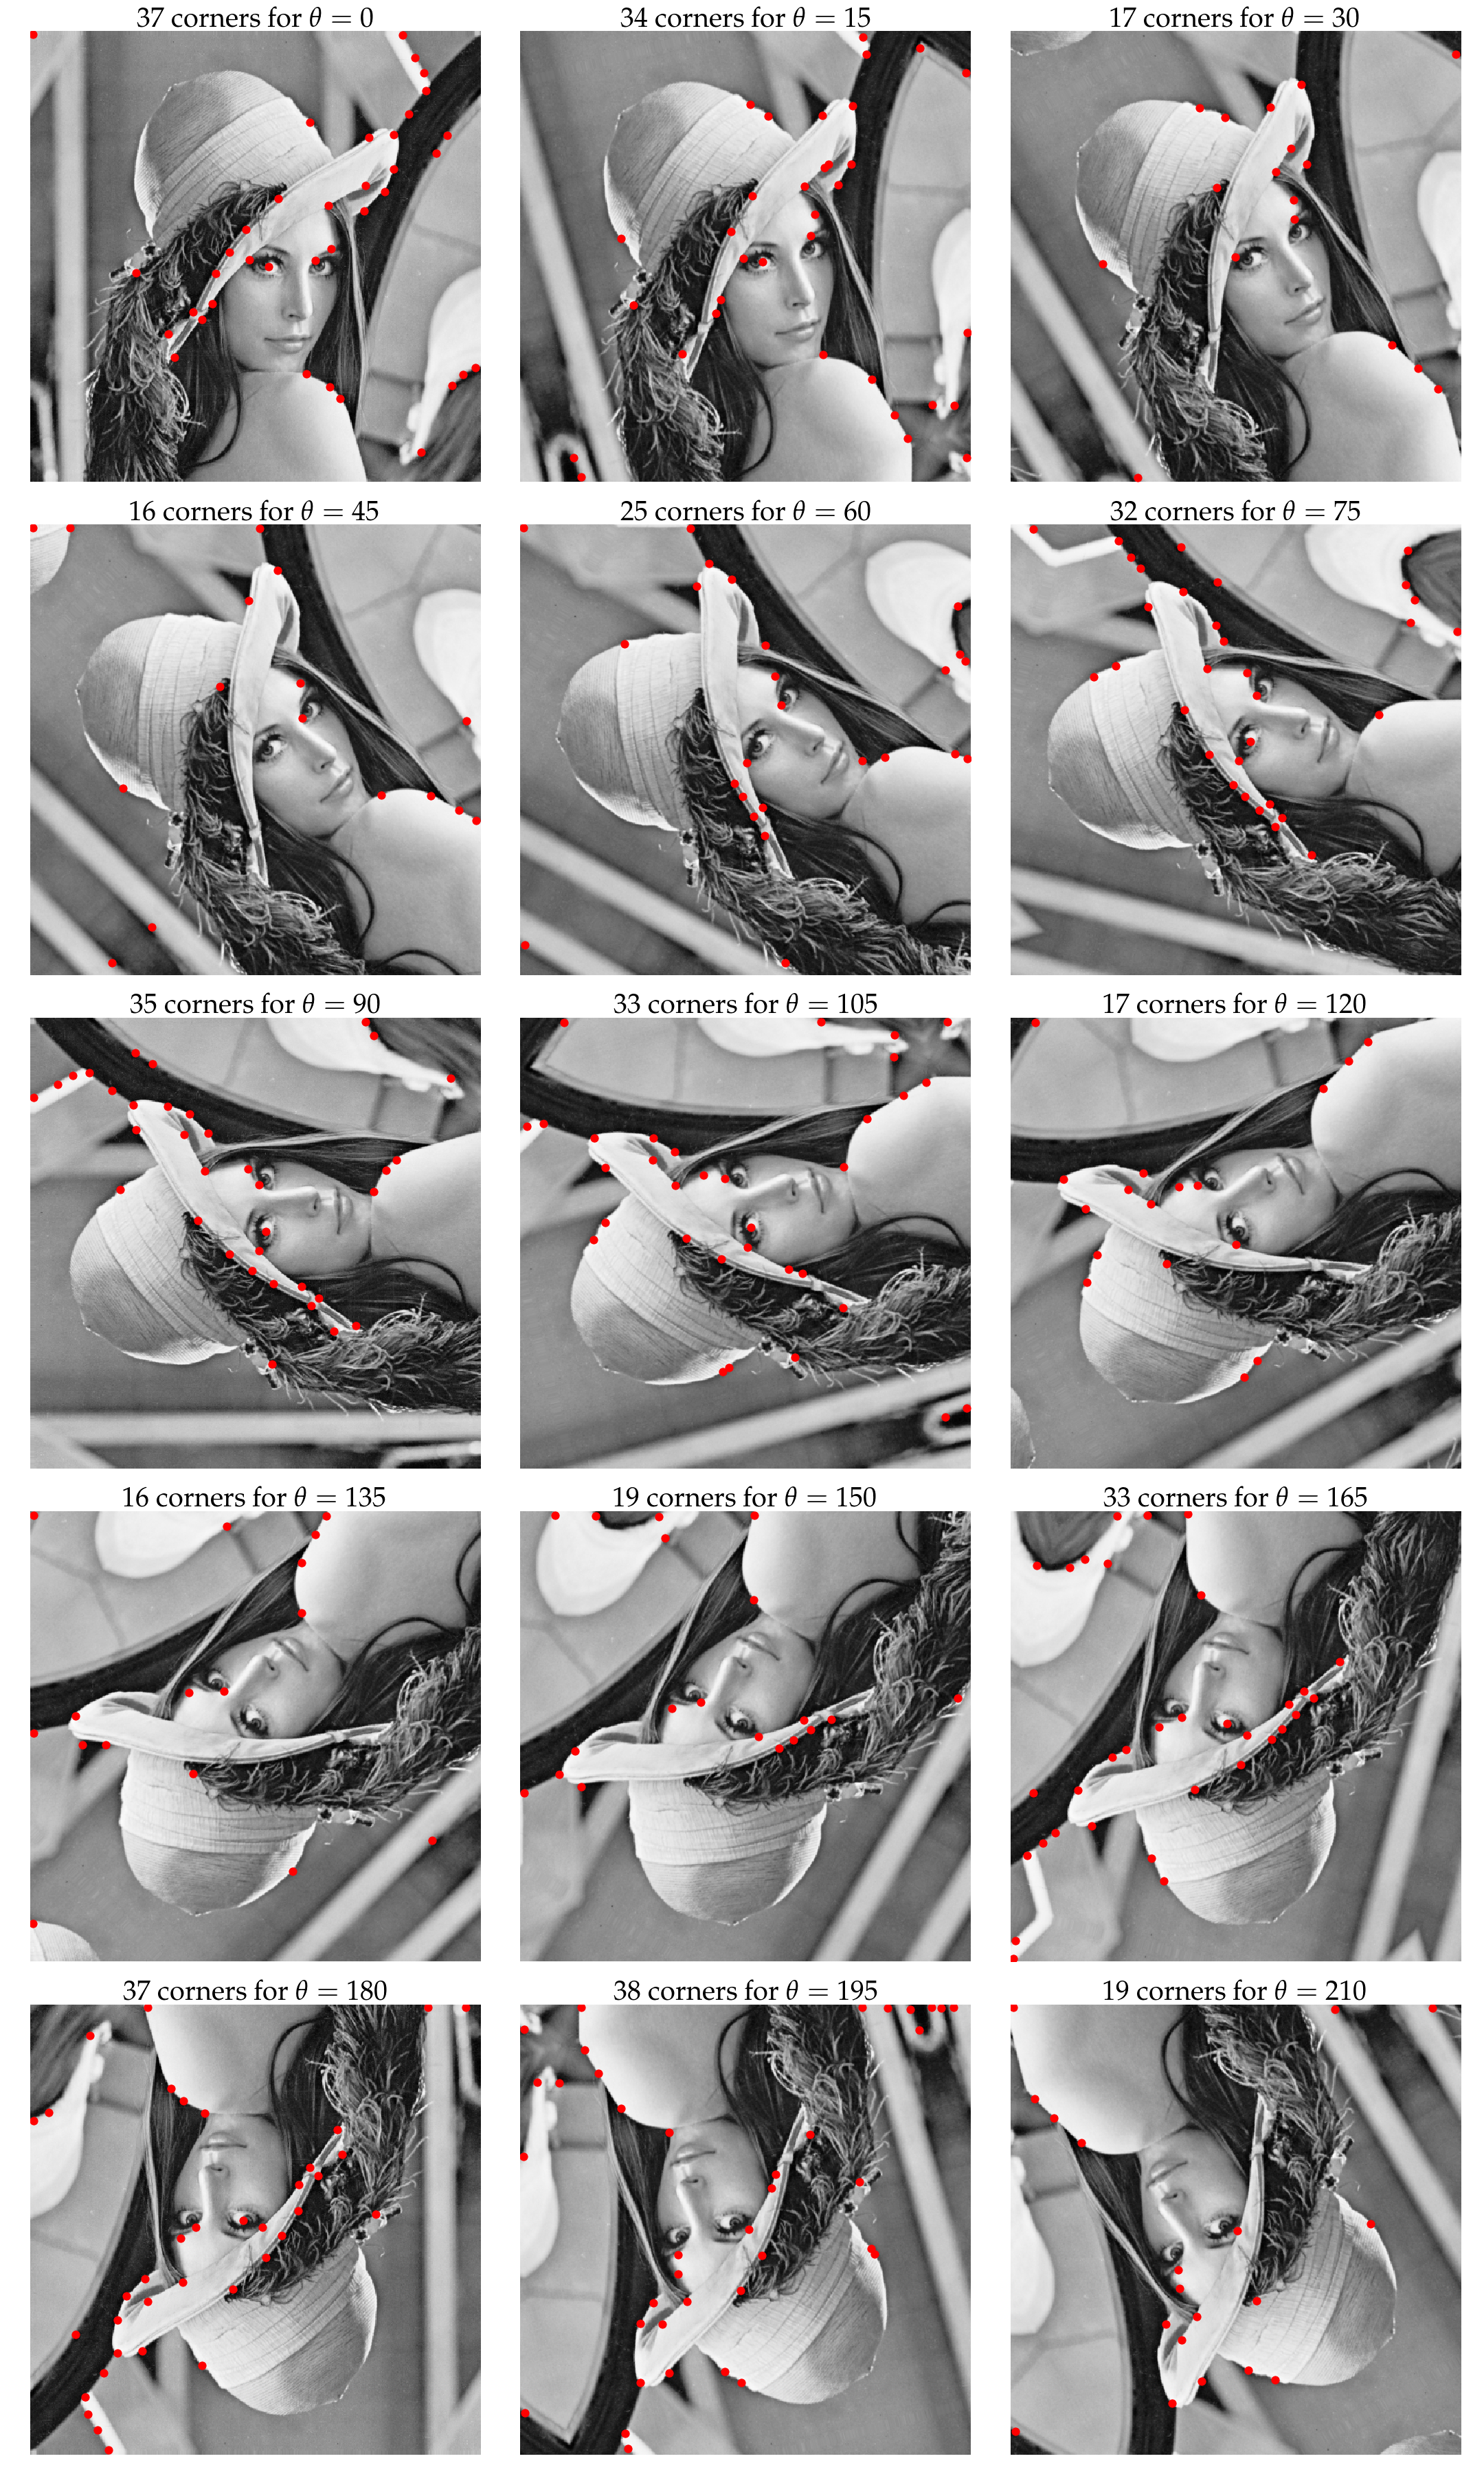
\includegraphics[height = 0.9\textheight]{3_lena_raw}
	\caption{Sensibilité aux rotations des détections, effectuées sans \textit{anms}}
	\label{fig_3_rot_lena_raw}
\end{figure}

\subsection{Au bruit}

La sensibilité au bruit est illustrée en figure~\ref{fig_3_noise_cameraman_raw} où le détecteur a été utilisé sur l'image Cameraman sans \textit{anms}, image à laquelle a été rajouté un bruit gaussian de moyenne nulle et d´écart-type \(\sigma_n \in [0, 80]\). On rappelle que l'image est encodée sur 256 niveau de gris. On constate que le nombre de détection, ainsi que leur position, restent très similaires, jusqu'à \(\sigma_n = 80\) : le détecteur conçu est donc robuste à l'ajout de bruit blanc.

\begin{figure}[H]
	\centering
	\includegraphics[width = 0.9\textwidth]{3_cameraman_raw}
	\caption{Sensibilité au bruit des détections, effectuées sans \textit{anms}}
	\label{fig_3_noise_cameraman_raw}
\end{figure}


\subsection{Au changement d'échelle}

La robustesse aux changement d'échelle a été mesurée qualitativement en figure~\ref{fig_3_rescale} où le détecteur a été utilisé sur l'image Lena sans \textit{anms}, pour différentes échelles simulées, de \(0.5\) à \(4.5\). On constate une grande disparité sur le nombre de détections effectuées, qui présente un maximum, dans le cas étudié, pour une image aggrandie 2 fois, avec \(139\) détections, alors qu'on partait de 30 détections pour le facteur \(0.5\) et qu'on en détecte pratiquement autant pour un facteur \(4.5\).


\begin{figure}[H]
	\centering
	\includegraphics[width = 0.9\textwidth]{3_lena_rescale_raw}
	\caption{Sensibilité au bruit des détections, effectuées sans \textit{anms}}
	\label{fig_3_rescale}
\end{figure}


\section{Changement de point de vue}

LLe détecteur a été utilisé sur une série d'images toutes issues d'une même scène, mais à laquelle on a appliqué différentes homographies générées aléatoirement.

\begin{figure}[H]
	\centering
	\includegraphics[width = 0.9\textwidth]{4_views_raw}
	\caption{Sensibilité au changement des détections du point de vue de l'image, vis-à-vis de ce dernniers,
\end{figure}

\end{document}
